\documentclass[border=10pt]{standalone}

\usepackage{tikz}
\usepackage{tikzsymbols}
\usetikzlibrary{calc,patterns,shapes.geometric}

\def\centerarc[#1](#2)(#3:#4:#5){\draw[#1] ($(#2)+({#5*cos(#3)},{#5*sin(#3)})$) arc (#3:#4:#5);}

\begin{document}
	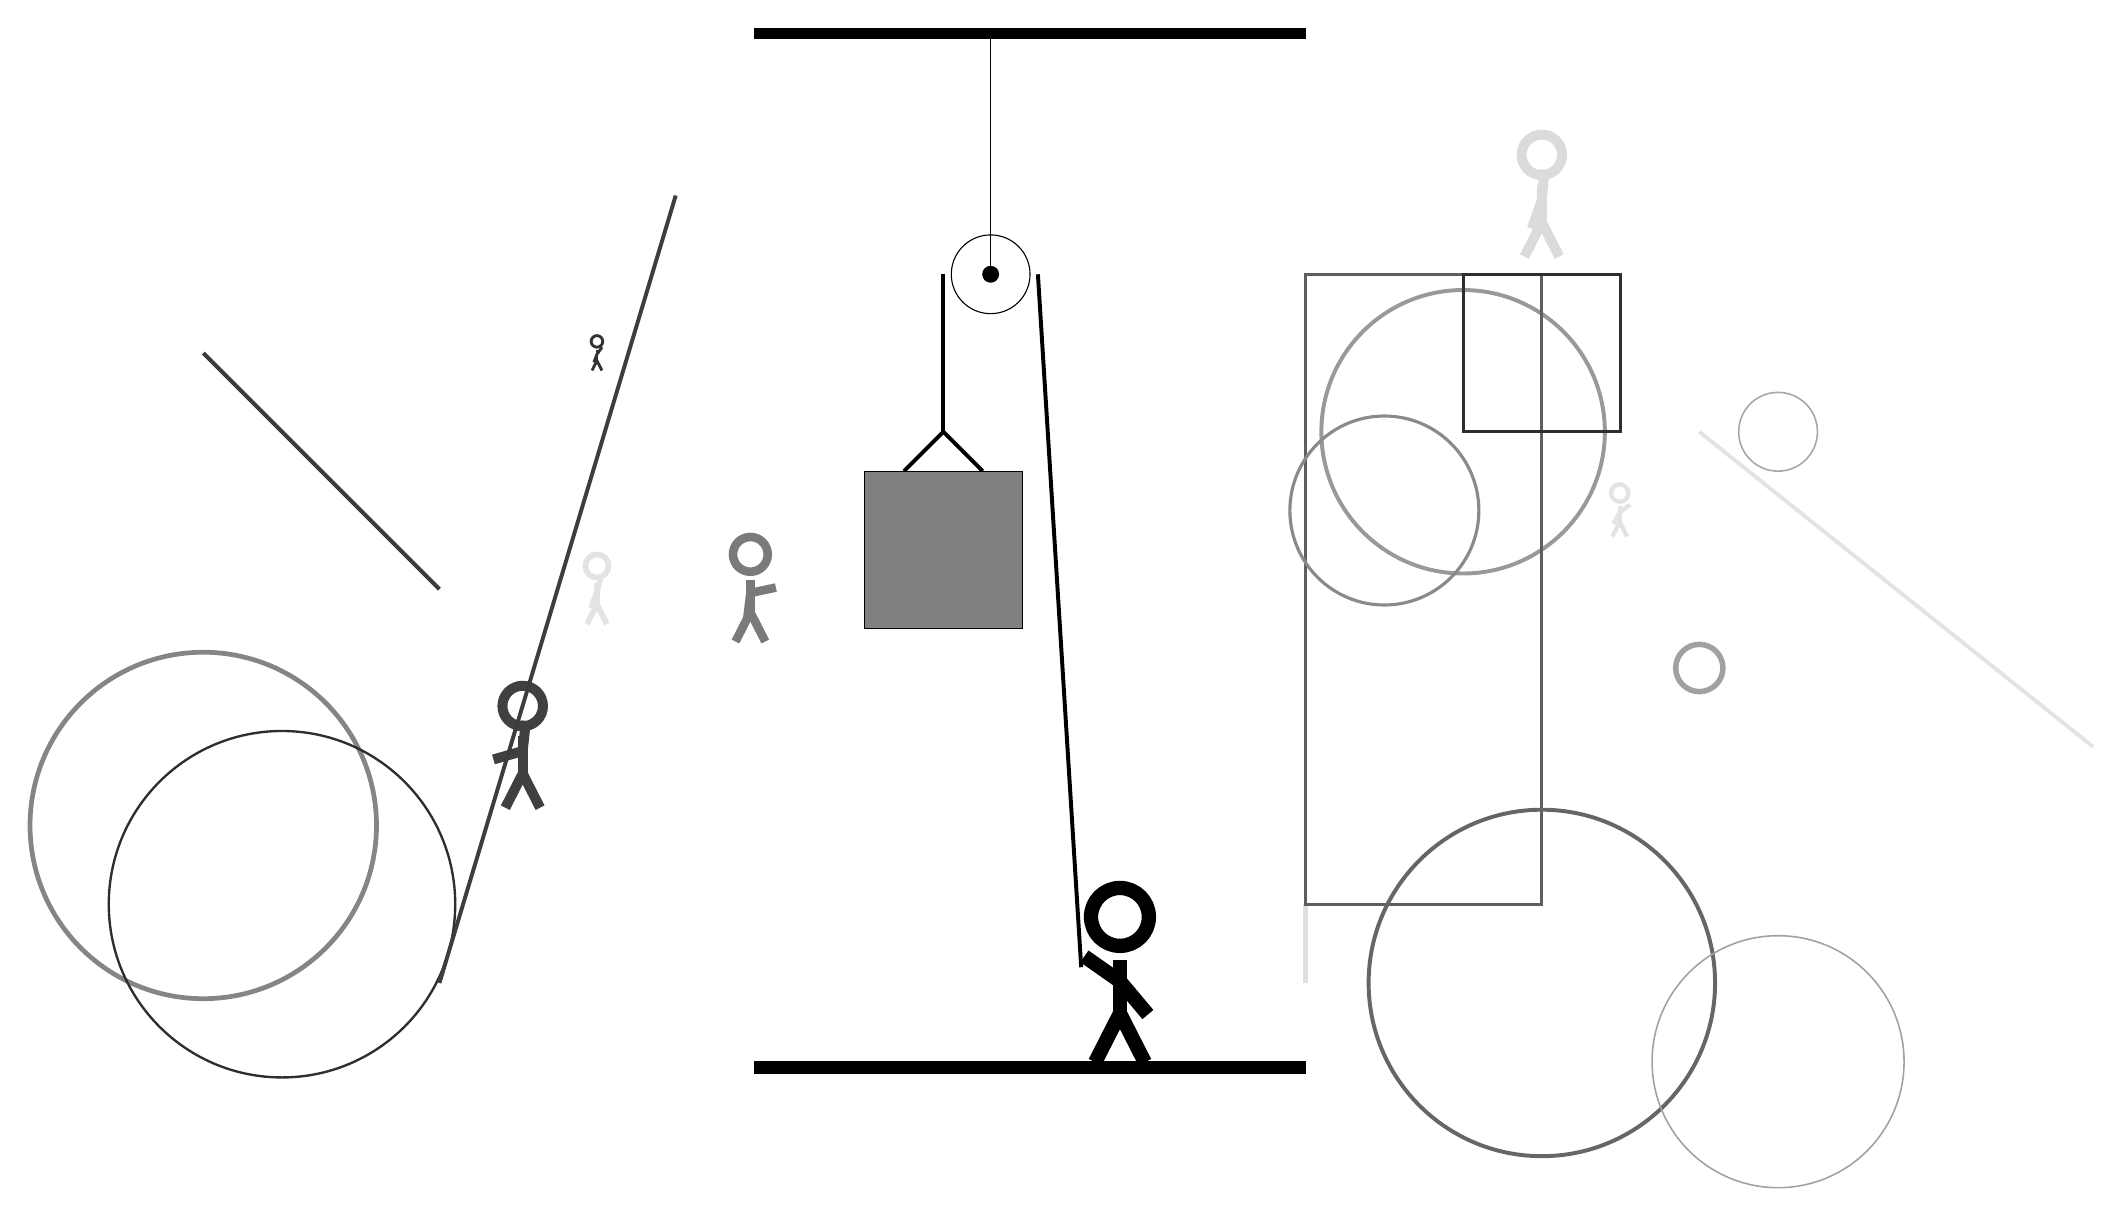
\begin{tikzpicture}
		%%%%% START %%%%%
		
		\draw[fill=black] (-2, 10) rectangle (5, 10.125);
		
		\draw (1, 7) circle (0.5);
		\draw[fill=black] (1, 7) circle (0.1);
		\draw (1, 10) -- (1, 7);
		
		\draw[line width=0.5mm] (-0.1, 4.5) -- (0.4, 5.0) -- (0.9, 4.5);
		\draw[fill=black!50] (-0.6, 4.5) rectangle (1.4, 2.5);
		
		\draw[line width=0.5mm] (0.4, 7) -- (0.4, 5.0);
		\centerarc[line width=0.5mm](1, 7)(0:180:0.6);
		\draw[line width=0.5mm](1.6, 7) -- (2.15, -1.8);
		
		\node at (2.6, -1.9) {\Strichmaxerl[10][-35][-50]};
		
		\draw [line width=0.5mm, color=black!40](7, 5) circle (1.8);
		
		\node[line width=0.2mm, color=black!52] at (-2, 3) {\Strichmaxerl[6][83][12]};
		\draw [line width=0.2mm, color=black!35](11, 5) circle (0.5);
		\node[line width=0.3mm, color=black!11] at (-4, 3) {\Strichmaxerl[4][70][76]};
		
		\draw[line width=0.5mm, color=black!11](10, 5) -- (15, 1);
		\draw [line width=0.6mm, color=black!48](-9, 0) circle (2.2);
		\draw[line width=0.7mm, color=black!12] (5, -1) rectangle (5, -2);
		
		\draw [line width=0.7mm, color=black!37](10, 2) circle (0.3);
		\node[line width=0.2mm, color=black!14] at (8, 8) {\Strichmaxerl[7][71][85]};
		
		\node[line width=0.6mm, color=black!80] at (-4, 6) {\Strichmaxerl[2][69][54]};
		\draw[line width=0.4mm, color=black!63] (5, -1) rectangle (8, 7);
		
		\draw [line width=0.5mm, color=black!60](8, -2) circle (2.2);
		\draw[line width=0.4mm, color=black!82] (7, 7) rectangle (9, 5);
		
		\draw [line width=0.3mm, color=black!82](-8, -1) circle (2.2);
		\node[line width=0.6mm, color=black!11] at (9, 4) {\Strichmaxerl[3][61][37]};
		\node[line width=0.6mm, color=black!75] at (-5, 1) {\Strichmaxerl[7][16][84]};
		
		\draw [line width=0.4mm, color=black!46](6, 4) circle (1.2);
		
		\draw[line width=0.5mm, color=black!76](-6, 3) -- (-9, 6);
		\draw[line width=0.5mm, color=black!76](-6, -2) -- (-3, 8);
		\draw [line width=0.2mm, color=black!37](11, -3) circle (1.6);
		
		\draw[fill=black] (-2, -3) rectangle (5, -3.15);
		
		%%%%% END %%%%%
	\end{tikzpicture}
\end{document}